\documentclass[hidelinks,12pt]{article}
\usepackage[left=0.25cm,top=1cm,right=0.25cm,bottom=1cm]{geometry}
%\usepackage[landscape]{geometry}
\textwidth = 20cm
\hoffset = -1cm
\usepackage[utf8]{inputenc}
\usepackage[spanish,es-tabla, es-lcroman]{babel}
\usepackage[autostyle,spanish=mexican]{csquotes}
\usepackage[tbtags]{amsmath}
\usepackage{nccmath}
\usepackage{amsthm}
\usepackage{amssymb}
\usepackage{mathrsfs}
\usepackage{graphicx}
\usepackage{subfig}
\usepackage{caption}
%\usepackage{subcaption}
\usepackage{standalone}
\usepackage[outdir=./Imagenes/]{epstopdf}
\usepackage{siunitx}
\usepackage{physics}
\usepackage{color}
\usepackage{float}
\usepackage{hyperref}
\usepackage{multicol}
\usepackage{multirow}
%\usepackage{milista}
\usepackage{anyfontsize}
\usepackage{anysize}
%\usepackage{enumerate}
\usepackage[shortlabels]{enumitem}
\usepackage{capt-of}
\usepackage{bm}
\usepackage{mdframed}
\usepackage{relsize}
\usepackage{placeins}
\usepackage{empheq}
\usepackage{cancel}
\usepackage{pdfpages}
\usepackage{wrapfig}
\usepackage[flushleft]{threeparttable}
\usepackage{makecell}
\usepackage{fancyhdr}
\usepackage{tikz}
\usepackage{bigints}
\usepackage{menukeys}
\usepackage{tcolorbox}
\tcbuselibrary{breakable}
\usepackage{scalerel}
\usepackage{pgfplots}
\usepackage{pdflscape}
\pgfplotsset{compat=1.16}
\spanishdecimal{.}
\renewcommand{\baselinestretch}{1.5} 
\renewcommand\labelenumii{\theenumi.{\arabic{enumii}})}

\newcommand{\python}{\texttt{python}}
\newcommand{\textoazul}[1]{\textcolor{blue}{#1}}
\newcommand{\azulfuerte}[1]{\textcolor{blue}{\textbf{#1}}}
\newcommand{\funcionazul}[1]{\textcolor{blue}{\textbf{\texttt{#1}}}}

\newcommand{\pderivada}[1]{\ensuremath{{#1}^{\prime}}}
\newcommand{\sderivada}[1]{\ensuremath{{#1}^{\prime \prime}}}
\newcommand{\tderivada}[1]{\ensuremath{{#1}^{\prime \prime \prime}}}
\newcommand{\nderivada}[2]{\ensuremath{{#1}^{(#2)}}}


\newtheorem{defi}{{\it Definición}}[section]
\newtheorem{teo}{{\it Teorema}}[section]
\newtheorem{ejemplo}{{\it Ejemplo}}[section]
\newtheorem{propiedad}{{\it Propiedad}}[section]
\newtheorem{lema}{{\it Lema}}[section]
\newtheorem{cor}{Corolario}
\newtheorem{ejer}{Ejercicio}[section]

\newlist{milista}{enumerate}{2}
\setlist[milista,1]{label=\arabic*)}
\setlist[milista,2]{label=\arabic{milistai}.\arabic*)}
\newlength{\depthofsumsign}
\setlength{\depthofsumsign}{\depthof{$\sum$}}
\newcommand{\nsum}[1][1.4]{% only for \displaystyle
    \mathop{%
        \raisebox
            {-#1\depthofsumsign+1\depthofsumsign}
            {\scalebox
                {#1}
                {$\displaystyle\sum$}%
            }
    }
}
\def\scaleint#1{\vcenter{\hbox{\scaleto[3ex]{\displaystyle\int}{#1}}}}
\def\scaleoint#1{\vcenter{\hbox{\scaleto[3ex]{\displaystyle\oint}{#1}}}}
\def\scaleiiint#1{\vcenter{\hbox{\scaleto[3ex]{\displaystyle\iiint}{#1}}}}
\def\bs{\mkern-12mu}

\newcommand{\Cancel}[2][black]{{\color{#1}\cancel{\color{black}#2}}}


\usepackage[siunitx]{circuitikz}
\usetikzlibrary{patterns, arrows, decorations.markings}
\definecolor{ashgrey}{rgb}{0.7, 0.75, 0.71}

\author{M. en C. Gustavo Contreras Mayén. \texttt{gux7avo@ciencias.unam.mx} \\
M en C. Abraham Lima Buendía. \texttt{abraham3081@ciencias.unam.mx}}
\title{Examen Final Primera Vuelta 2024-1 \\ {\large Curso Física Computacional}}
\date{ }
\begin{document}

\maketitle
\fontsize{14}{14}\selectfont

\textbf{Instrucciones: } Resuelve cada ejercicio apoyándote con un código en python. Debes de incluir los correspondientes módulos que ocupes. Dentro de cada archivo con la solución NO deben de incluirse las funciones de módulos. Se recomienda el uso de archivos .py más que notebook de Jupyter.

\begin{enumerate}
% \item Calcula todas las raíces positivas de las siguientes expresiones mediante el método de la secante con una tolerancia de $\num{d-3}$:
% \begin{enumerate}
% \item $\tan (x) - x + 1 = 0, \hspace{1.5cm} 0 < x < 3 \pi$
% \item $\sin (x) - 0.3 \, e^{x} = 0, \hspace{1.5cm} x > 0$
% \item $x + \dfrac{1}{(x + 3) x} = 0$
% \end{enumerate}
\item La masa $m$ está unida a un resorte de longitud libre $b$ y rigidez $k$.
\begin{figure}[H]
\centering
\begin{tikzpicture}
    \tikzstyle{spring}=[thick, decorate,
                        decoration={zigzag, pre length=0.3cm, 
                        post length=0.3cm, segment length=9}]
    \draw (0, 0) rectangle (5, 0.25);
    \draw [loosely dashdotted] (0, 0.125) -- (5, 0.125);
    \draw (0.0, -0.15) [pattern= north east lines] rectangle (-0.4, 0.4);
    \draw (5.0, -0.15) [pattern= north east lines] rectangle (5.4, 0.4);
    \draw (3, -0.2) rectangle (3.5, 0.5);
    \node at (3.6, -0.4) {$m$};
    \draw [stealth-stealth] (0.5, 0.125) -- (0.5, -3) node [left, midway] {$b$};
    \draw (0.3, -3) -- (0.7, -3);
    \draw (0.7, -3) [pattern= north east lines] rectangle (1.2, -3.5);
    \draw[spring] (0.95, -3) -- (3.25, 0.125) node [below, yshift=-1.5cm, xshift=-0.5cm] {$k$};
    \draw (0.95, 0.8) -- (0.95, -3);
    \draw (3.25, 0.2) -- (3.25, 0.8);
    \draw [stealth-stealth] (0.95, 0.7) -- (3.25, 0.7) node [above, midway] {$x$};
\end{tikzpicture}
\end{figure}
El coeficiente de fricción entre la masa y la barra horizontal es $\mu$. Se puede demostrar que la aceleración de la masa es $\ddot{x} = - f (x)$, donde:
\begin{align*}
f (x) = \mu \, g + \dfrac{k}{m} ( \mu \, b + x) \left( 1 - \dfrac{b}{\sqrt{b^{2} + x^{2}}} \right)
\end{align*}
Si la masa se libera del reposo en $x = b$, su velocidad en $x = 0$ está dada por:
\begin{align*}
v_{0} = \sqrt{2 \scaleint{6ex}_{\bs 0}^{b} f (x) \dd{x}}
\end{align*}
Calcula $v_{0}$ mediante integración numérica usando: $m = \SI{0.8}{\kilo\gram}$, $b = \SI{0.4}{\metre}$, $\mu = 0.3$, $k = \SI{80}{\newton\per\metre}$ y $g = \SI[per-mode=symbol]{9.81}{\metre\per\square\second}$.
\item Una corriente alterna está descrita por:
\begin{align*}
i (t) = i_{0} \left( \sin \dfrac{\pi \, t}{t_{0}} \right) - \beta \, \sin \dfrac{2 \, \pi \, t}{t_{0}}
\end{align*}
donde $i_{0} = \SI{1}{\ampere}$, $t_{0} = \SI{0.05}{\second}$ y $\beta = 0.2$. Calcula la raíz media cuadrática de la corriente, que se define como:
\begin{align*}
i_{\text{rmc}} = \sqrt{\dfrac{1}{t_{0}} \scaleint{6ex}_{\bs 0}^{t_{0}} i^{2} (t) \dd{t}}
\end{align*}
\item (\textbf{2 puntos}) Considera el siguiente sistema:
\begin{figure}[H]
\centering
\begin{tikzpicture}
    \tikzstyle{spring}=[thick, decorate,
                        decoration={zigzag, pre length=0.3cm, 
                        post length=0.3cm, segment length=6}]
    \tikzstyle{damper}=[thick,decoration={markings,  
                        mark connection node=dmp,
                        mark=at position 0.5 with 
                        {
                          \node (dmp) [thick,inner sep=0pt,transform shape,rotate=-90,minimum
                      width=15pt,minimum height=3pt,draw=none] {};
                          \draw [thick] ($(dmp.north east)+(2pt,0)$) -- (dmp.south east) -- (dmp.south
                      west) -- ($(dmp.north west)+(2pt,0)$);
                          \draw [thick] ($(dmp.north)+(0,-5pt)$) -- ($(dmp.north)+(0,5pt)$);
                        }
                      }, decorate]

    \draw (0, 0) [pattern= north east lines] rectangle (5, 0.25);
    \draw (0, 0) [pattern= north east lines] rectangle (-0.25, 2);
    \draw (2.5, 0.5) rectangle (4.5, 2.1) node [pos=0.5] {$m$};
    \draw (2.7, 0.375) circle (3.2pt);
    \draw (4.2, 0.375) circle (3.2pt);
    \draw [spring] (0, 1.7) -- (2.5, 1.7) node [above, midway] {$k$};
    \draw [damper] (0, 0.8) -- (2.5, 0.8) node [above, midway,pos=0.3] {$c$};
\end{tikzpicture}
\end{figure}

La ecuación diferencial que describe el movimiento del sistema masa-resorte-amortiguador es:
\begin{align*}
\ddot{y} + \dfrac{c}{m} \, \dot{y} + \dfrac{k}{m} \, y = 0
\end{align*}
donde $m = \SI{2}{\kilo\gram}$, $c = \SI{460}{\newton\second\per\metre}$ y $k = \SI{450}{\newton\per\metre}$. Las condiciones iniciales son $y (0) = \SI{0.01}{\metre}$ y $\dot{y} (0) = 0$.
\begin{enumerate}
\item Demuestra que este es un problema rígido.
\item Determina un valor de $h$ que se usaría en integración numérica con el método no adaptativo de Runge-Kutta.
\item Realiza la integración de $t = 0$ a $\SI{0.2}{\second}$ con la $h$ elegida.
\item Grafica $\dot{y}$ contra $t$.
\item Integra ahora con el método adaptativo de Runge-Kutta de $t = 0$ a $\SI{0.2}{\second}$.
\item Grafique $\dot{y}$ contra $t$.
\item Discute tus resultados.
\end{enumerate}
\item Un cilindro grueso transporta un fluido con una temperatura de $\SI{0}{\celsius}$. Al mismo tiempo, el cilindro se sumerge en un baño que se mantiene a $\SI{200}{\celsius}$.
\begin{figure}[H]
    \centering
    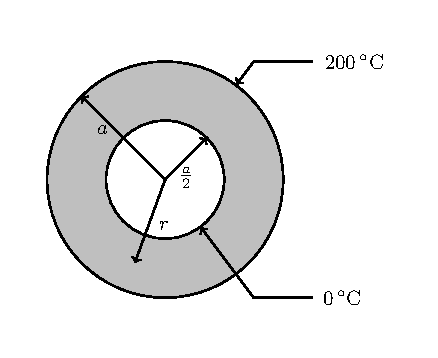
\includegraphics[scale=1]{fig_edo_cdf_cilindro_01.eps}
\end{figure}
La ecuación diferencial y las CDF que determinan la conducción de calor en estado estacionario en el cilindro son:
\begin{align*}
\dv[2]{T}{r} = -\dfrac{1}{r} \, \dv{T}{r} \hspace{1cm} \eval{T}_{r = \dfrac{a}{2}} = \SI{0}{\celsius} \hspace{1cm} \eval{T}_{r = a} = \SI{200}{\celsius}
\end{align*}
donde $T$ es la temperatura.

Determina el perfil de temperatura a través del cilindro usando el método de diferencias finitas, compara tu resultado con la solución analítica:
\begin{align*}
T =  \SI{200}{\celsius} \, \left( 1 - \dfrac{\ln r/a}{\ln 0.5} \right)
\end{align*}
% \item Considera el siguiente circuito eléctrico:
% \begin{figure}[H]
%     \centering
%     \begin{circuitikz}
%         \draw (0, 0) to[L, l=$L$] (2,0);
%         \draw (2, 0) to[L, l=$L$] (4,0);
%         \draw (4, 0) to[L, l=$L$] (6,0);
%         \draw (6, 0) to[L, l=$L$] (8,0);
%         \draw (0, 0) to[cC, l=$C$] (0, -2);
%         \draw (2, 0) to[cC, l=$\dfrac{C}{2}$] (2, -2);
%         \draw (4, 0) to[cC, l=$\dfrac{C}{3}$] (4, -2);
%         \draw (6, 0) to[cC, l=$\dfrac{C}{4}$] (6, -2);
%         \draw (8, 0) to[cC, l=$\dfrac{C}{5}$] (8, -2);
%         \draw (0, -2) -- (8, -2);
%     \end{circuitikz}
% \end{figure}
% Apoyándote con la ley de Kirchoff para la corriente, plantea las correspondientes ecuaciones para las corrientes en cada malla, luego calcula las frecuencias angulares de las corrientes.
% \item Considera el siguiente circuito eléctrico:
% \begin{figure}[H]
%     \centering
%     \begin{circuitikz}
%         \draw (0, 0) to[cC, l=$C$] (2,0);
%         \draw (2, 0) to[cC, l=$\dfrac{C}{2}$] (4,0);
%         \draw (4, 0) to[cC, l=$\dfrac{C}{3}$] (6,0);
%         \draw (6, 0) to[cC, l=$\dfrac{C}{4}$] (8,0);
%         \draw (0, 0) to[L, l=$L$] (0, -2);
%         \draw (2, 0) to[L, l=$L$] (2, -2);
%         \draw (4, 0) to[L, l=$L$] (4, -2);
%         \draw (6, 0) to[L, l=$L$] (6, -2);
%         \draw (8, 0) to[L, l=$L$] (8, -2);
%         \draw (0, -2) -- (8, -2);
%     \end{circuitikz}
% \end{figure}
% Apoyándote con la ley de Kirchoff para la corriente, plantea las correspondientes ecuaciones para la corrientes en cada malla, luego calcula las frecuencias angulares de las corrientes.
\item Considera el siguiente sistema mecánico:
\begin{figure}[H]
\centering
\begin{tikzpicture}
    \tikzstyle{spring}=[thick, decorate,
                        decoration={zigzag, pre length=0.3cm, 
                        post length=0.3cm, segment length=6}]
    \draw [fill, color=ashgrey] (0, 0) rectangle (9.6, 0.25);
    \draw (0, 0.25) -- (9.6, 0.25);
    \draw [fill, color=ashgrey] (0, 0) rectangle (-0.25, 2);
    \draw (0, 0.25) -- (0, 2);
    \draw [spring] (0, 1.1) -- (1.5, 1.1) node [above, midway] {$k$};
    \draw (1.5, 0.5) rectangle (2.5, 1.6) node [pos=0.5] {$m_{1}$};
    \draw (1.7, 0.4) circle (3.5pt);
    \draw (2.3, 0.4) circle (3.5pt);
    \draw (2.5, 1.7) -- (2.5, 2.3);
    \draw [-stealth] (2.5, 2.1) -- (3.1, 2.1) node [above, pos=1.10] {$u_{1}$};
    \draw [spring] (2.5, 1.1) -- (4, 1.1) node [above, midway] {$k$};
    \draw (4, 0.5) rectangle (5, 1.6) node [pos=0.5] {$m_{2}$};
    \draw (4.2, 0.4) circle (3.5pt);
    \draw (4.8, 0.4) circle (3.5pt);
    \draw (5, 1.7) -- (5, 2.3);
    \draw [-stealth] (5, 2.1) -- (5.6, 2.1) node [above, pos=1.10] {$u_{2}$};
    \draw [spring] (5, 1.1) -- (6.5, 1.1) node [above, midway] {$k$};

    \draw [spring] (6.8, 1.1) -- (8.3, 1.1) node [above, midway] {$k$};
    \draw (8.3, 0.5) rectangle (9.3, 1.6) node [pos=0.5] {$m_{n}$};
    \draw (8.5, 0.4) circle (3.5pt);
    \draw (9.1, 0.4) circle (3.5pt);
    \draw (9.3, 1.7) -- (9.3, 2.3);
    \draw [-stealth] (9.3, 2.1) -- (9.9, 2.1) node [above, pos=1.10] {$u_{n}$};
\end{tikzpicture} 
\end{figure}
El sistema de ecuaciones diferenciales del sistema de masas-resortes son:
\begin{align*}
k (- 2 \, u_{1} + u_{2}) &= m_{1} \, \ddot{u} \\
k (u_{i-1} - 2 \, u_{i} + u_{i+1}) &= m_{i} \, \ddot{u}_{i} \hspace{1.5cm} i = 2, 3, \ldots, n - 1 \\
k (u_n-1) &= m_{n} \, \ddot{u}_{n}
\end{align*}
donde $u_{i} (t)$ es el desplazamiento de su punto de equilibrio de la masa $i$, el valor $k$ es la constante del resorte. Dados $k$ y las masas:
\begin{align*}
m = \big[ m_{1} \quad m_{2} \quad \ldots \quad m_{n} \big]^{T}
\end{align*}
\begin{enumerate}
\item Elabora un código que calcule las $N$ frecuencias angulares más pequeñas del sistema y los correspondientes desplazamientos de las masas.
\item Ejecuta el programa con $N = 2$, $k = \SI{500}{\kilo\newton\per\metre}$ y
\begin{align*}
\vb{m} = \big[ 1.0 \quad 1.0 \quad 1.0 \quad 8.0 \quad 1.0 \quad 1.0 \quad 8.0 \big]^{T} \,\, \text{kg}
\end{align*}
\end{enumerate}
\end{enumerate}
\end{document}